\section{Experiments}
\label{sec:experiments}

We evaluate stagnation detection across four axes: in-domain accuracy, cross-agent transfer, robustness to design choices, and temporal dynamics of labeling functions.
All reported metrics are evaluated against silver labels derived from majority vote over three labeling functions (\S\ref{sec:method}).

\paragraph{Circular evaluation caveat.}
Structural features (command repetition ratios, file operation counts, edit distances) are computed from the same signals that the labeling functions use to produce silver labels.
Consequently, the in-domain structural F1 of 0.9951 reflects an upper bound on how well these features can \emph{reverse-engineer} the labeling functions, not detection accuracy against true ground truth.
The cross-agent evaluation on OpenHands (0.967 macro-F1) is non-circular: models trained on SWE-Agent LF distributions are tested on a different agent whose LF firing patterns differ substantially (\S\ref{sec:cmd_rep_ablation}).
A human-annotated gold set provides the definitive non-circular evaluation (\S\ref{sec:gold_set}).

%-------------------------------------------------------------------
\subsection{Experimental Setup}
\label{sec:setup}

\paragraph{Datasets.}
We extract sliding windows of $k{=}5$ consecutive actions from agent trajectories.
\textbf{SWE-Agent} trajectories from SWE-bench \citep{jimenez2024swebench,yang2024sweagent} yield 54,809 windows with a stagnation ratio of 28.5\%.
\textbf{OpenHands} (OH) trajectories \citep{wang2025openhands} yield 150,652 windows with a stagnation ratio of 6.6\%.
Silver labels are produced by majority vote over three labeling functions; confidence equals the number of agreeing LFs (1--3).
Unless stated otherwise, evaluation uses the conf${\geq}$2 subset: $N{=}1{,}824$ for SWE-Agent (485 stagnation, 1,339 progress) and $N{=}43{,}376$ for OH.

\begin{table}[t]
\centering
\small
\begin{tabular}{llrrc}
\toprule
\textbf{Agent} & \textbf{Source} & \textbf{Windows} & \textbf{Stag\,\%} & \textbf{Conf${\geq}$2} \\
\midrule
SWE-Agent & SWE-bench & 54,809 & 28.5 & 15,401 \\
OpenHands & CodeAct   & 150,652 & 6.6 & 43,376 \\
\bottomrule
\end{tabular}
\caption{Dataset statistics. Stagnation ratios differ substantially across agents, reflecting different action distributions.}
\label{tab:dataset_stats}
\end{table}

\paragraph{Detection methods.}
(1)~\textbf{Structural features}: 30 hand-crafted features (repetition rates, file operation counts, edit distances, output entropy) fed to Logistic Regression (LR), Random Forest (RF), and Gradient Boosting (GB).
(2)~\textbf{ProgressProbe}: Qwen3-Embedding-0.6B \citep{zhang2025qwen3embedding} embeddings (1024-dim) processed by a 2-layer GRU \citep{cho2014gru} with attention \citep{bahdanau2015attention} (hidden$=$256, dropout$=$0.1), early-stopped at epoch~3 with patience~5.
(3)~\textbf{Mean-pool + LR}: Mean-pooled Qwen3 embeddings with logistic regression.
(4)~\textbf{LLM-as-Judge}: Claude Sonnet zero-shot window-level classification (\$11.66 API cost for the SWE test set).
(5)~\textbf{Cosine similarity}: Cosine distance between consecutive window embeddings with a validation-tuned threshold.

\paragraph{Metrics.}
Macro-F1 is the primary metric. We also report per-class F1 for stagnation (F1\textsubscript{stag}) and progress (F1\textsubscript{prog}).

%-------------------------------------------------------------------
\subsection{Main Results}
\label{sec:main_results}

Table~\ref{tab:main_results} presents in-domain results on the SWE-Agent conf${\geq}$2 test set and cross-agent transfer to OpenHands.

\begin{table*}[t]
\centering
\small
\begin{tabular}{l ccc cc}
\toprule
& \multicolumn{3}{c}{\textbf{SWE-Agent In-Domain} (conf${\geq}$2)} & \multicolumn{2}{c}{\textbf{OpenHands Transfer}} \\
\cmidrule(lr){2-4} \cmidrule(lr){5-6}
\textbf{Method} & Macro-F1 & F1\textsubscript{stag} & F1\textsubscript{prog} & All & Conf${\geq}$2 \\
\midrule
Structural RF$^\dagger$       & \textbf{0.9951} & 0.9928 & 0.9974 & 0.9123 & \textbf{0.9959} \\
Structural GB$^\dagger$       & \textbf{0.9951} & 0.9928 & 0.9974 & \textbf{0.9674} & \underline{0.9919} \\
Structural LR$^\dagger$       & 0.9874 & 0.9815 & 0.9933 & 0.7801 & 0.9671 \\
ProgressProbe (GRU)           & \underline{0.9055} & 0.8593 & 0.9518 & 0.5280 & --- \\
\quad + full OH fine-tune      & ---    & ---    & ---    & 0.7510 & --- \\
Mean-pool + LR                & 0.8435 & 0.7620 & 0.9250 & ---    & --- \\
LLM-as-Judge                  & 0.6625 & 0.6055 & 0.7195 & ---    & --- \\
Cosine Similarity             & 0.5606 & ---    & ---    & ---    & --- \\
\bottomrule
\end{tabular}
\caption{Stagnation detection results. In-domain evaluation on SWE-Agent conf${\geq}$2 test set ($N{=}1{,}824$) and zero-shot cross-agent transfer to OpenHands. $^\dagger$Structural metrics are evaluated against LF-derived labels and reflect LF-reconstructibility rather than ground-truth accuracy (see circular evaluation caveat). Best in \textbf{bold}, second-best \underline{underlined}.}
\label{tab:main_results}
\end{table*}

In-domain, structural RF achieves 0.9951 macro-F1, exceeding the GRU probe by 8.96 percentage points (pp) and the LLM judge by 33.3\,pp.
However, the structural--probe gap is inflated by circular evaluation: structural features reconstruct the LFs that generated the labels.
The more informative comparison is among non-circular methods: the GRU probe outperforms mean-pool~+~LR by 6.2\,pp, confirming that temporal modeling within windows adds value beyond static embedding aggregation.
The LLM judge underperforms all learned methods despite substantially higher cost.

%-------------------------------------------------------------------
\subsection{Cross-Agent Transfer}
\label{sec:cross_agent}

Table~\ref{tab:main_results} (right columns) shows models trained on SWE-Agent and evaluated on OpenHands without any OH training data.
Structural GB transfers best, achieving 0.967 macro-F1 on all OH windows---21.6\,pp above the probe fine-tuned on 100\% of OH data (0.751).
RF drops to 0.912 on all-confidence OH data despite matching GB in-domain, suggesting GB's boosted ensemble is more robust to distributional shift.
Both structural models recover to $>$0.99 on conf${\geq}$2 OH windows, where label noise is lower.

The probe's zero-shot transfer (0.528) is near chance, and even full OH fine-tuning only reaches 0.751.
This asymmetry---structural features transfer naturally while learned embeddings do not---is a central empirical finding: stagnation manifests in action-level structure that generalizes across agents.

\paragraph{Multi-seed stability.}
Structural RF: $0.9951{\pm}0.0000$ in-domain (3 seeds, zero variance); GB cross-agent: $0.9678{\pm}0.0015$.
The probe shows higher variance: $0.9185{\pm}0.0113$, though all seeds exceed 0.90.

%-------------------------------------------------------------------
\subsection{Robustness Analysis}
\label{sec:robustness}

\paragraph{Encoder ablation.}
Replacing Qwen3-0.6B with BGE-M3 \citep{chen2024bgem3} or E5-large-v2 \citep{wang2024e5} yields probe macro-F1 of 0.9413 and 0.9363, respectively (vs.\ 0.9055 for Qwen3).
All encoders exceed 0.90, indicating the probe's temporal architecture, not a specific encoder, drives performance. Full results appear in Appendix Table~\ref{tab:encoder_ablation}.

\paragraph{Window size.}
$k{=}5$ is optimal (0.9309 macro-F1); $k{=}3$ drops 5.9\,pp and $k{=}7$ drops 1.8\,pp.
Shorter windows lack sufficient context; longer windows dilute signal by spanning both progress and stagnation phases.
Details in Appendix Table~\ref{tab:window_ablation}.

\paragraph{Data scaling.}
Figure~\ref{fig:data_scaling} shows probe performance scales monotonically from 0.8054 (10\% training data) to 0.9055 (100\%), with structural RF providing a ceiling at 0.9951 (dashed line).
The curve has not plateaued, suggesting larger trajectory corpora could further close the structural--probe gap.

\begin{figure}[t]
\centering
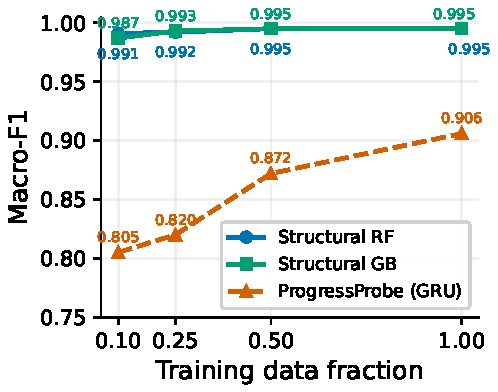
\includegraphics[width=\columnwidth]{../../figures/paper/fig_data_scaling.pdf}
\caption{Probe macro-F1 vs.\ training data fraction. Structural RF ceiling shown as dashed line. Performance scales monotonically but has not saturated at 100\% data.}
\label{fig:data_scaling}
\end{figure}

%-------------------------------------------------------------------
\subsection{Labeling Function Temporal Dynamics}
\label{sec:lf_temporal}

We analyze when each LF first fires relative to the onset of stagnation episodes (Table~\ref{tab:lf_temporal}, Figure~\ref{fig:lf_temporal}).

\begin{table}[t]
\centering
\small
\begin{tabular}{lrrrr}
\toprule
\textbf{LF} & \textbf{Lag} & \textbf{Lead\,\%} & \textbf{Conc.\,\%} & \textbf{Lag\,\%} \\
\midrule
cmd\_rep      & $-1.87$ & 36.1 & --- & --- \\
file\_diff    & $-1.20$ & 17.1 & --- & --- \\
outcome\_bp   & $+6.70$ & ---  & --- & 48.4 \\
\bottomrule
\end{tabular}
\caption{Temporal roles of labeling functions on SWE-Agent. Lag = mean steps relative to stagnation onset (negative = leading). Kruskal-Wallis $H{=}274.3$, $p{=}2.74{\times}10^{-60}$; all pairwise comparisons significant after Bonferroni correction.}
\label{tab:lf_temporal}
\end{table}

The three LFs occupy distinct temporal niches.
Command repetition leads stagnation onset by 1.87 steps on average, making it an early warning signal.
File diff is near-concurrent ($-1.20$ steps).
Outcome backpropagation lags by 6.70 steps, acting as a retrospective confirmation.

All pairwise differences are significant (Kruskal-Wallis $H{=}274.3$, $p{=}2.74{\times}10^{-60}$; Bonferroni-corrected pairwise: cmd\_rep vs.\ file\_diff $p{=}1.44{\times}10^{-26}$, cmd\_rep vs.\ outcome\_bp $p{=}6.67{\times}10^{-39}$, file\_diff vs.\ outcome\_bp $p{=}3.47{\times}10^{-47}$).

\paragraph{Cross-agent reversal.}
On OpenHands, cmd\_rep shifts from leading ($-1.87$) to lagging ($+3.32$ steps).
This reversal explains the cmd\_rep pathology analyzed in \S\ref{sec:cmd_rep_ablation}: OH's action distribution triggers cmd\_rep on progress windows, inverting its diagnostic value.

\begin{figure}[t]
\centering
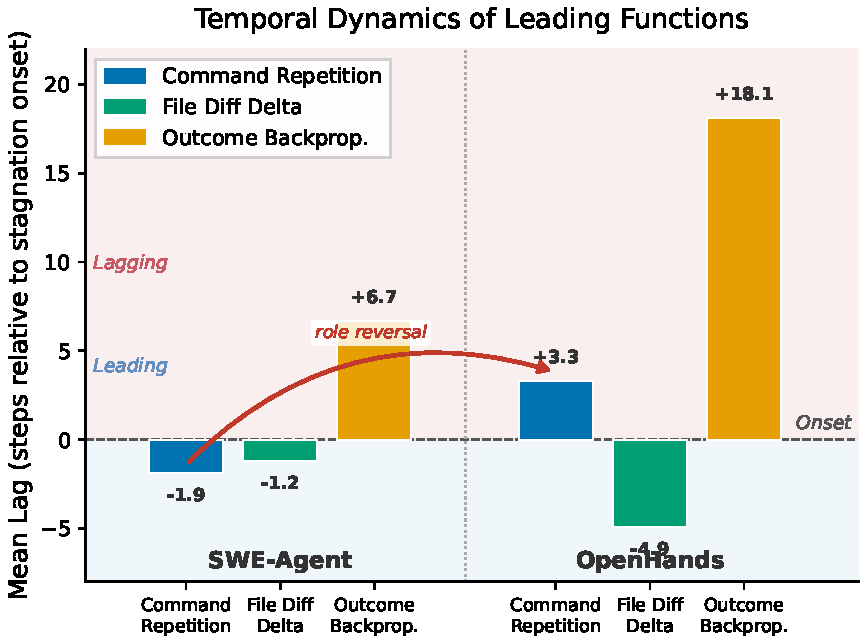
\includegraphics[width=\columnwidth]{../../figures/paper/fig_lf_temporal.pdf}
\caption{Temporal roles of labeling functions relative to stagnation onset on SWE-Agent. cmd\_rep leads ($-1.87$ steps), file\_diff is near-concurrent ($-1.20$), outcome\_bp lags ($+6.70$). Inset: OH reversal where cmd\_rep becomes lagging.}
\label{fig:lf_temporal}
\end{figure}

%-------------------------------------------------------------------
\subsection{Command Repetition Ablation}
\label{sec:cmd_rep_ablation}

The cmd\_rep LF fires on 92.3\% of OH windows (vs.\ 65.6\% on SWE-Agent), with a 71\% false positive rate on OH progress windows.
Table~\ref{tab:cmd_rep_ablation} shows the effect of removing it.

\begin{table}[t]
\centering
\small
\begin{tabular}{lcccc}
\toprule
\textbf{LF Config} & \textbf{ZS F1} & \textbf{FT F1} & \textbf{FT F1\textsubscript{s}} & \textbf{FT F1\textsubscript{p}} \\
\midrule
3-LF (w/ cmd\_rep) & 0.530 & 0.751 & 0.544 & 0.959 \\
2-LF (no cmd\_rep) & 0.607 & \textbf{0.927} & 0.938 & 0.917 \\
\midrule
$\Delta$ & +7.7\,pp & +17.6\,pp & +39.4\,pp & $-4.2$\,pp \\
\bottomrule
\end{tabular}
\caption{Effect of removing cmd\_rep on OpenHands probe performance. ZS = zero-shot transfer from SWE-Agent; FT = fine-tuned on 100\% OH data. F1\textsubscript{s}/F1\textsubscript{p} = stagnation/progress F1.}
\label{tab:cmd_rep_ablation}
\end{table}

Removing cmd\_rep improves zero-shot transfer by 7.7\,pp and fine-tuned performance by 17.6\,pp.
The gain is driven almost entirely by stagnation recall (+39.4\,pp F1\textsubscript{stag}), at a modest cost to progress detection ($-4.2$\,pp F1\textsubscript{prog}).
The 3-LF fine-tuned model's stagnation F1 of 0.544 reveals that cmd\_rep corrupts silver labels so thoroughly that even full fine-tuning on OH data cannot recover.
This motivates agent-specific LF selection: labeling functions validated on one agent architecture may become adversarial on another.

%-------------------------------------------------------------------
\subsection{Temporal Label Models}
\label{sec:temporal_label_models}

We investigate whether incorporating LF temporal dynamics into label aggregation improves over majority vote (MV).
Table~\ref{tab:temporal_models} compares three temporal label models \citep{ratner2017snorkel,safranchik2020linkedhmm}.

\begin{table}[t]
\centering
\small
\begin{tabular}{lccc}
\toprule
\textbf{Method} & \textbf{Conf${\geq}$2 F1} & \textbf{MV Agr.} & \textbf{Probe F1$^\ddagger$} \\
\midrule
MV (baseline) & 0.8946$^\ast$ & 1.000 & 0.8468 \\
TWV ($\sigma{=}2$) & \textbf{0.9003} & 0.885 & 0.8211 \\
Lag-HMM & 0.8936 & 0.820 & --- \\
HMM & 0.7502 & 0.685 & 0.6564 \\
\bottomrule
\end{tabular}
\caption{Temporal label model comparison. $^\ast$MV conf${\geq}$2 F1 is a self-evaluation baseline (MV evaluated against itself on high-confidence windows). $^\ddagger$Downstream: probe trained on each method's labels, evaluated on SWE-Agent conf${\geq}$2 vs.\ MV labels.}
\label{tab:temporal_models}
\end{table}

TWV achieves the highest conf${\geq}$2 F1 (0.9003, +0.57\,pp over MV), but this gain does not propagate downstream: a probe trained on TWV labels scores 0.8211 vs.\ 0.8468 for MV-trained ($-2.57$\,pp).
TWV flips 14.1\% of conf$=$1 labels, introducing noise that hurts probe training.
HMM overpredicts stagnation (29,176 stagnation vs.\ 25,633 progress windows), degrading downstream performance to 0.6564.
Lag-HMM closely tracks MV ($-0.1$\,pp) despite explicitly modeling temporal offsets, suggesting that the temporal structure captured by individual LFs does not improve \emph{aggregation}.

\paragraph{TWV sensitivity.}
The Gaussian kernel bandwidth $\sigma$ is critical: $\sigma{=}2$ is optimal (0.9003); $\sigma{=}1$ drops to 0.8105 and $\sigma{\geq}5$ falls below 0.81.
This narrow operating range, combined with the downstream degradation, makes TWV impractical as a drop-in MV replacement.

These results constitute a negative finding: despite clear temporal structure in LF firing patterns (\S\ref{sec:lf_temporal}), temporal label models do not improve over simple majority vote for downstream stagnation detection.

%-------------------------------------------------------------------
\subsection{Gold Set Validation}
\label{sec:gold_set}
\goldset{Human-annotated gold set (650 windows) validation pending. Results will be added upon completion (expected 2026-05-17). This provides the non-circular ground truth evaluation for all methods.}
